%%%%%%%%%%%%%%%%%%%%%%%%%
\section{\label{sec:common_issues}Implementation issues in MC molecular simulations}
%%%%%%%%%%%%%%%%%%%%%%%%%

Although the derivation of the acceptance criteria for MC trials is the focus of this article, common errors encountered during the implementation of MC are included here.
For a more comprehensive discussion of the inner workings of MC see Ref.~\cite{dubbeldam_inner_2013}.
Thus, the scope of this section is for testing MC trial implementations.
In this section, we discuss energy tests and machine precision issues for helping to capture common errors, the calculation of standard deviations using the block method \cite{flyvbjerg_error_1989, grossfield_best_2018}, the generation of a random position on the surface of a unit sphere and spherical shell, and the generation of random rotation matrices.
This section then ends with a discussion of the general workflow for testing a new MC trial.

%%%%%%%%%%%%%%%%%%%%%%%%%
\subsection{\label{sec:energy_test}Energy tests and machine precision}
%%%%%%%%%%%%%%%%%%%%%%%%%

MC often involves the perturbation of a subset of the system instead of the entire system.
Only the energy of interaction of the perturbed particles needs to be computed to obtain the change in the energy of the system.
The energy of the system after a trial is accepted is the previous energy of the system plus the change.
This energy is referred to as the running total energy.
However, round off errors at the limit of numerical precision cause the running total energy to be different from the total energy calculated based on the interactions of all the particles.
This difference increases with the number of trials.
It is recommended to infrequently compute the energy of the entire system and compare the total energy with the running total energy from each energy change.
The total energy may also be compared and updated during trials which update all the particles, such as volume changes.
If the relative differences are not within an acceptable tolerance based on machine precision and the magnitude of the total energy, then this is a clear indication there is a problem with the way that the change in energy was computed, and an error or warning should be made visible.
If the relative difference is within an acceptable tolerance, the running total energy is then reset to the newly calculated value and the simulation continues.

Another recommended test is to not use any optimizations when infrequently computing the total energy of the entire system as part of the energy test described above.
Infrequent in this context essentially means much less often than once every $N$ trials, where $N$ is the total number of particles, assuming each trial moves individual particles, such that the computational cost of the trials is much greater than the computational cost of the infrequent and unoptimized total energy calculations.
If this unoptimized calculation of the entire system is done infrequently, it will not slow down the simulation significantly.
But it will serve as a test of the optimizations and may reveal issues with neighbor or cell lists, for example.

Machine precision round off errors may cause a number of other problems.
One that is frequently encountered in software implementations of MC is the acceptance probabilities.
Acceptance probabilities may involve several factors which are both big and small.
For this reason, it is best to compute and store acceptance probabilities as the natural logarithm, $\ln\chi$, and not $\chi$ \cite{shah_cassandra_2017}.
Machine precision issues may also appear when selecting among Rosenbluth weights.
In the FEASST \cite{hatch_monte_2024} implementation, overflow is avoided by shifting by a constant inside the exponential terms based on the maximum value, and later correcting for the shift.
Also, the total Rosenbluth factor may reveal if there is a very small chance for the trial to be accepted.
In that case, the trial may be outright rejected, because machine precision can make it difficult to select from among the poor choices.

%%%%%%%%%%%%%%%%%%%%%%%%%
\subsection{\label{sec:code}Additional code}
%%%%%%%%%%%%%%%%%%%%%%%%%

The following three sections contain Python code examples that were used in this article.
The first is for computing standard deviations of the mean using block averaging, which was utilized in the ideal gas tests to compare ensemble average properties with theoretical expectations.
The second is for randomly generating positions on a unit sphere, which is used for orienting molecules and anisotropic particles.
The third is for randomly generating positions in a spherical shell, which is used in AVB algorithms.

%%%%%%%%%%%%%%%%%%%%%%%%%
\subsubsection{\label{sec:block_av}Block averages}
%%%%%%%%%%%%%%%%%%%%%%%%%

In the example shown in Code Block~\ref{sim:statistics}, the standard deviation is computed using the blocking method \cite{flyvbjerg_error_1989}.
In this case, only blocks of $100$ samples are considered, but a careful analysis would show that the resulting standard deviation is independent of the block size (when large enough).
Thus, with this implementation, we are assuming that the sampled states are independent after $100$ MC trials, which may be reasonable for an ideal gas but most likely not for a dense liquid.
See the blocking tutorial in python interface of FEASST \cite{hatch_monte_2024} for an example with computing the block standard deviation from the average position of a particle randomly walking in one dimension with periodic boundary conditions.
If the maximum translation is smaller than the periodic boundary, correlations in the position may persist over many trials.

\begin{figure}
\lstinputlisting[
language=Python,
label={sim:statistics},
caption={The statistics module computes the mean and the standard deviation of the mean using blocks.}
]{../codes/statistics.py}
\end{figure}

%%%%%%%%%%%%%%%%%%%%%%%%%
\subsubsection{\label{sec:unit_sphere}Random position on a unit sphere surface and random orientation}
%%%%%%%%%%%%%%%%%%%%%%%%%

%In the example shown in Code Block~\ref{sim:unit_sphere}, positions are generated uniformly on the surface of a sphere.
%This is an important case to consider, because MC trials often assume that particles may be randomly oriented.
%However, one must be careful in how an orientation is generated.
%Uniformly selected values of Euler angles, for example, will result in a bias along the poles.
%Code Block~\ref{sim:quaternion} also shows how quaternions may be randomly generated to represent a uniformly random point on the surface of a sphere \cite{vesely_angular_1982}.
%Code Block~\ref{sim:rotationmatrix} uses these randomly generated quaternions to compute rotation matrices.
%A randomly generated perturbation of orientation is then demonstrated in Fig.~\ref{fig:random_orientation}.
Situations arise where one needs to generate a point at random uniformly on the surface of a sphere in 3D.  This is equivalent to defining an isotropically random direction or a randomly oriented unit vector. There are several ways to approach this: (1) sample the spherical coordinates $\theta$ and $\phi$, appropriately weighted; (2) use a rejection method to generate a point uniformly inside a sphere, i.e., repeatedly sample in a cube that circumscribes the sphere until the sample is also in the sphere, and then normalize the sampled point to a unit vector; (3) sample the $x$, $y$ and $z$ coordinates on independent Gaussian distributions, which yields a point sampled from a spherically symmetric 3D probability density, and normalize to a unit vector. The first method listed here is illustrated in Code Block~\ref{sim:unit_sphere}.

A similar problem is sampling a quaternion, which may be interpreted as a point on the surface of a unit 4D-hypersphere.
Accordingly, Code Block~\ref{sim:quaternion} shows how quaternions may be randomly generated by sampling uniformly on the surface of a 4D hypersphere using an efficient rejection method \cite{vesely_angular_1982}.
Code Block~\ref{sim:rotationmatrix} uses these randomly generated quaternions to compute rotation matrices, which could be used to generate a fully random orientation by rotating from an arbitrary reference orientation.
Finally, a randomly generated perturbation of orientation is shown using the axis-angle method in Code Block~\ref{sim:random_orientation} and Fig.~\ref{fig:random_orientation}.

\begin{figure}
\lstinputlisting[
language=Python,
label={sim:unit_sphere},
caption={The unit\_sphere module generates randomly uniform positions on the surface of a unit sphere in three dimensions.}
]{../codes/unit_sphere.py}
\end{figure}

\begin{figure}
\lstinputlisting[
language=Python,
label={sim:quaternion},
caption={The quaternion module generates a random quaternion by sampling on the surface of a 4-dimensional hypersphere.}
]{../codes/quaternion.py}
\end{figure}

\begin{figure}
\lstinputlisting[
language=Python,
label={sim:rotationmatrix},
caption={The rotation module generates a rotation matrix from an axis and angle or a quaternion. The first index is the row and the second index is the column, each starting with an index of zero.}
]{../codes/rotation.py}
\end{figure}

\begin{figure}
\lstinputlisting[
language=Python,
label={sim:random_orientation},
caption={Visualize randomly uniform perturbations in three dimensional particle orientations.}
]{../codes/random_orientation.py}
\end{figure}

\begin{figure}
\begin{centering}
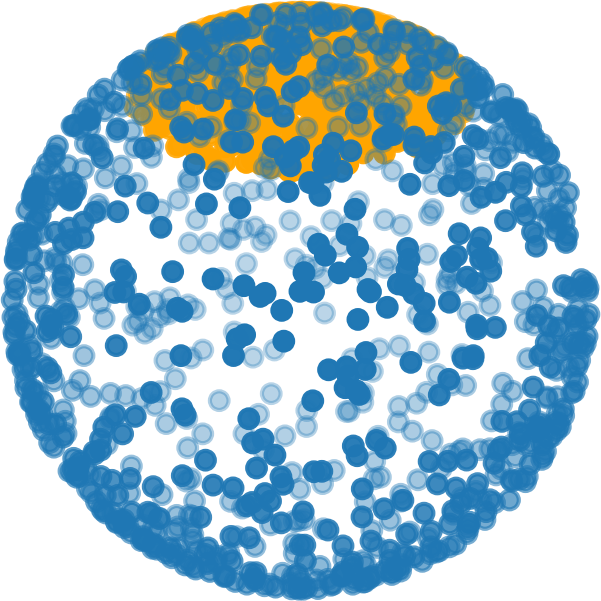
\includegraphics[width=8.5cm]{../figures/random_orientation.png}
\caption{
The output from Code Block~\ref{sim:random_orientation} shows $10^3$ uniformly random blue unit vectors emanating from the origin.
The other $10^3$ orange unit vectors are confined to the top hemisphere because they were randomly generated with the axis-angle method by perturbing the orientation of an upwards $z$-axis vector (shown in black) with a maximum angle parameter, $\delta \theta_{max}=\pi=180$ degrees.
\label{fig:random_orientation}
}
\end{centering}
\end{figure}

%%%%%%%%%%%%%%%%%%%%%%%%%
\subsubsection{\label{sec:spherical_shell}Uniform position in a spherical shell}
%%%%%%%%%%%%%%%%%%%%%%%%%

In the example shown in Code Block~\ref{sim:spherical_shell}, positions are generated uniformly within a spherical shell.
This is used to generate new trial positions with the AV of target isotropic sites, as shown in Fig.~\ref{fig:spherical_shell}.

\begin{figure}
\lstinputlisting[
language=Python,
label={sim:spherical_shell},
caption={Visualize randomly uniform positions in a spherical shell in three dimensions.}
]{../codes/spherical_shell.py}
\end{figure}

\begin{figure}
\begin{centering}

\includegraphics[width=8.5cm]{../figures/spherical_shell.png}
\caption{
Example output from Code Block~\ref{sim:spherical_shell} shows approximately $10^5$ small blue points randomly generated inside a spherical shell of outer radius $3$ and inner radius $2$.
To see the inside cavity, points above $z=0$ were removed.
\label{fig:spherical_shell}
}
\end{centering}
\end{figure}

%%%%%%%%%%%%%%%%%%%%%%%%%
\subsection{\label{sec:testingnewtrial}Workflow for testing a new MC trial}
%%%%%%%%%%%%%%%%%%%%%%%%%

Another recommendation during testing of new trials is to start with a result that was obtained using an established and well-tested set of trials and known to high confidence.
One source of such results is the National Institute of Standards and Technology (NIST) standard reference simulation website \cite{shen_nist_2017}.
Another choice is to generate results with one or more well-tested, open-source simulation codes.
Then, when computing the same result with the new trial, any differences may be further investigated.
Start with the simplest model and thermodynamic conditions that may reveal differences, such as an ideal gas simulation.
Also, if possible, completely remove as many other trials from the simulation with the new trial, thereby allowing one to better determine if the new trial is incorrect.
Otherwise, the difference in the results due to the new trial may be difficult to detect, or the impact of the new trial difficult to isolate, because the other trials are contributing greatly.
For example, AVB insertions and deletions can be tested without standard insertions and deletions, and without even $NVT$ translation and rotation trials.
